\documentclass[border=5pt]{standalone}

\usepackage{tikz}

\begin{document}
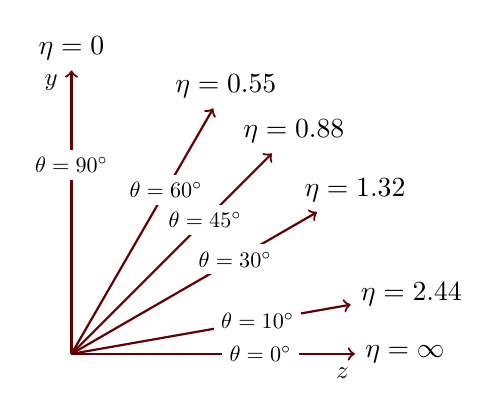
\begin{tikzpicture}[scale=3]
 
  % limits
  \def\R{1.2}
 
  % axis labels
  \node[scale=0.9,below=5pt,left=2pt] at (0,\R) {$y$};
  \node[scale=0.9,left=5pt,below=2pt] at (\R,0) {$z$};
 
  % lines
  \foreach \t/\e in {90/0,60/0.55,45/0.88,30/1.32,10/2.44,0/\infty}{
    \draw[->,black!60!red,thick]
      (0,0) -- ({\R*cos(\t)},{\R*sin(\t)})
      node[anchor=180+\t,black] {$\eta=\e$};
    \node[fill=white,scale=0.8] at ({0.8*cos(\t)},{0.8*sin(\t)}) {$\theta=\t^\circ$};
  }
 
\end{tikzpicture}
\end{document}
